%%%%%%%%%%%%%%%%%%%%%%%%%%%%%%%%%%%%%%%%%%%%%%%%%%%%%%%%%%%%%%%%%
%%% %
%%% % weiiszablon.tex
%%% % The Faculty of Electrical and Computer Engineering
%%% % Rzeszow University Of Technology diploma thesis Template
%%% % Szablon pracy dyplomowej Wydziału Elektrotechniki 
%%% % i Informatyki PRz
%%% % June, 2015
%%%%%%%%%%%%%%%%%%%%%%%%%%%%%%%%%%%%%%%%%%%%%%%%%%%%%%%%%%%%%%%%%

\documentclass[12pt,twoside]{article}

\usepackage{weiiszablon}

\author{Rafał Stępień}

\studentID{EF-169625}

\title{Książkowy dziennik w chmurze}
\titleEN{Cloud-based book journal}

\newcommand{\rodzajPracyNo}{1}


\supervisor{dr inż. Mariusz Mączka}

\supervisorEN{Dr. Eng. Mariusz Mączka}

\abstract{Treść streszczenia po polsku}
\abstractEN{Treść streszczenia po angielsku}

\begin{document}

\maketitle

\blankpage

\tableofcontents

\clearpage
\blankpage

\section{Wstęp}
W dobie rosnącej cyfryzacji i dynamicznego rozwoju technologii mobilnych, coraz więcej osób poszukuje
nowoczesnych narzędzi wspierających codzienne czynności, w tym także zarządzanie swoimi pasjami i 
zainteresowaniami. Jedną z takich pasji, cieszącą się niezmienną popularnością, jest czytanie książek.
Wraz z rosnącą liczbą dostępnych tytułów zarządzanie osobistą biblioteką może stać się problematyczne.

Niniejsza praca dotyczy zaprojektowania i implementacji aplikacji mobilnej o nazwie 
„BookTracker”, stworzonej z wykorzystaniem technologii Jetpack Compose 
oraz zintegrowanej z internetową bazą danych Supabase. Aplikacja oferuje użytkownikom możliwość 
oznaczania książek jako posiadanych lub przeczytanych, śledzenia nadchodzących premier 
literackich oraz zarządzania osobistą biblioteką w sposób przejrzysty i dostępny z każdego 
miejsca, dzięki wykorzystaniu technologii chmurowych. Tematyka ta została wybrana ze względu 
na rosnącą popularność aplikacji wspierających organizację życia codziennego oraz potrzebę 
zapewnienia użytkownikom narzędzi umożliwiających wygodne i efektywne zarządzanie ich kolekcjami 
literackimi.

Zakres pracy obejmuje zaprojektowanie kluczowych funkcji aplikacji, implementację interfejsu 
użytkownika oraz integrację z bazą danych w chmurze. Głównym celem pracy jest stworzenie aplikacji mobilnej, 
która w przejrzysty sposób umożliwi użytkownikom zarządzanie osobistą biblioteką książek z 
wykorzystaniem technologii chmurowych.

\clearpage

\section{Podobne aplikacje}

W dzisiejszych czasach niemal każda aplikacja ma już swoje odpowiedniki na rynku. Podczas 
tworzenia aplikacji postawiono więc na skupienie się na grupie docelowej użytkowników, którzy
oczekują konkretnych rozwiązań.

\subsection{Bookmory}

Bookmory to przykład wielu istniejących aplikacji dzięki którym można zarządzać swoją biblioteką, do jej
odpowiedników można zaliczyć jeszcze kilka aplikacji takich jak: StoryGraph, Bookshelf, czy Bookly.
Każda z wymienionych aplikacji spełnia podobne zadania, a dla większości użytkowników wybór pomiędzy nimi
nie ma większego znaczenia, ponieważ różnice między nimi są minimalne.

Istnienie tych aplikacji zainspirowało stworzenie alternatywy, która będzie różniła się od swoich
poprzedników unikalną funkcjonalnością i skupieniem się na konkretnej grupie odbiorców.

\subsection{TV Time}

TV Time to popularna aplikacja służąca do śledzenia postępu oglądania seriali i filmów. 
Pomimo tego, że aplikacja ta nie ma możliwości zarządzania książkami i skupia się wyłącznie na 
produkcjach filmowych, to funkcjonalność śledzenia seriali stała się inspiracją do stworzenia
alternatywnej aplikacji do śledzenia postępu czytania książek. Główną różnicą do 
istniejących już rozwiązań jest skupienie się na seriach książek wydawanych w tomach i ułatwieniu
użytkownikom obserwowania i zarządzania książkami, które są ze sobą powiązane.

\clearpage

\section{Środowiska i technologie}

Wybór odpowiednich środowisk i technologii jest kluczowym elementem każdego projektu informatycznego, 
ponieważ wpływa zarówno na efektywność pracy, jak i na jakość końcowego rozwiązania. Ważnym jest 
przedstawienie wybranych rozwiązań i uzasadnienie dlaczego były one wybrane zamiast alternatywnych
opcji.

\subsection{Android Studio}

Android Studio to oficjalne zintegrowane środowisko programistyczne (IDE) do tworzenia aplikacji na system
Android bazujące na IntelliJ IDEA firmy JetBrains, stworzone i rozwijane przez firmę Google. Jest to 
kompleksowe narzędzie, które oferuje zestaw funkcji, mających na celu ułatwienie tworzenia, debugowania i
publikowania aplikacji.

Środowisko to jest nieustannie aktualizowane przez Google, aby wspierać najnowsze wersje systemu Android
oraz dodawać nowe funkcje. Android Studio obsługuje programowanie w językach takich jak Java, Kotlin 
(rekomendowany przez Google), a także w mniejszym stopniu w C++.

Kluczowym elementem jest edytor kodu, który obsługuje autouzupełnianie, refaktoryzację oraz podpowiedzi 
kontekstowe, co znacząco ułatwia pisanie czystego i efektywnego kodu.

Android Studio zostało wybrane ze względu na to, że jest najpełniejszym narzędziem do tworzenia aplikacji
na system android i w przeciwieństwie do np. Visual Studio Code, można praktycznie od razu rozpocząć
pracę zamiast zajmowania się instalowaniem rozszerzeń i potrzebnych komponentów. Android Studio oferuje 
wszystkie niezbędne funkcje w jednym pakiecie.

\subsection{Kotlin}

Kotlin to nowoczesny, statycznie typowany język programowania, który został stworzony przez firmę 
JetBrains i jest oficjalnie wspierany przez Google do tworzenia natywnych aplikacji na system Android. 
Kotlin jest zaprojektowany z myślą o prostocie, bezpieczeństwie i interoperacyjności z Javą - język ten 
jest w pełni kompatybilny z istniejącym ekosystemem Javy, co umożliwia łatwą integrację z istniejącym kodem i 
bibliotekami.

Kotlin oferuje wiele nowoczesnych funkcji, które czynią go atrakcyjnym wyborem. Jego kluczowe 
cechy to m.in. zwięzła składnia, która pozwala na pisanie czytelnego i mniej podatnego na błędy kodu, oraz 
zaawansowane mechanizmy, takie jak obsługa funkcji wyższych rzędów, rozszerzenia klas czy programowanie funkcyjne. 
Wbudowane mechanizmy bezpieczeństwa, takie jak system typów zapobiegający błędom typu null pointer exception 
(tzw. "null safety"), znacząco zwiększają niezawodność aplikacji.

Kotlin wspiera także współbieżność dzięki korutynom, które są lekkim mechanizmem współbieżności umożliwiającym 
pisanie asynchronicznego kodu w czytelnym i intuicyjnym stylu. Korutyny działają w ramach istniejących wątków, 
wykorzystując mechanizmy wstrzymywania i wznawiania, co pozwala na efektywne zarządzanie zasobami systemowymi bez 
potrzeby blokowania wątków. To podejście znacząco upraszcza tworzenie wydajnych aplikacji, zwłaszcza tych, które 
intensywnie korzystają z asynchronicznej komunikacji sieciowej, przetwarzania dużych ilości danych czy operacji 
wejścia/wyjścia.

\subsection{Jetpack Compose}

Jetpack Compose to nowoczesny framework interfejsu użytkownika stworzony przez Google, który pozwala 
na tworzenie aplikacji na Androida w sposób deklaratywny. Zamiast używać tradycyjnych plików XML do 
definiowania widoków, Jetpack Compose umożliwia definiowanie interfejsu w kodzie Kotlin, co prowadzi 
do tworzenia prostszych, bardziej zwięzłych i łatwiejszych w utrzymaniu aplikacji.

Jedną z największych zalet Jetpack Compose jest możliwość dynamicznego reagowania na zmiany stanu aplikacji. 
Dzięki podejściu opartemu na deklaratywnej reaktywności, widoki automatycznie aktualizują się w odpowiedzi na 
zmiany danych, co eliminuje konieczność ręcznego zarządzania aktualizacjami interfejsu użytkownika.

W Jetpack Compose funkcje komponowalne (ang. composable functions) stanowią podstawę tworzenia interfejsu 
użytkownika. Są to specjalne funkcje oznaczone adnotacją @Composable, które pozwalają na deklaratywne definiowanie 
i łączenie elementów UI. Funkcje komponowalne w Jetpack Compose działają na zasadzie deklaratywnego określania 
struktury i zawartości interfejsu użytkownika, zamiast szczegółowego opisywania sposobu jego wyświetlania. Co 
umożliwia koncentrację na logice aplikacji, a nie na szczegółach implementacji interfejsu. Każda funkcja 
komponowalna może zawierać inne funkcje komponowalne, tworząc w ten sposób złożone i hierarchiczne struktury UI 
w sposób naturalny i łatwy do zrozumienia. Takie podejście umożliwia tworzeniee intuicyjnych, skalowalnych i łatwych 
w utrzymaniu aplikacji.

Jetpack Compose został wybrany, ponieważ jest rozwiązaniem w pełni zintegrowanym z Androidem, 
co zapewnia najlepszą optymalizację i wydajność w tworzeniu aplikacji natywnych na tę platformę.

\subsection{Material Design}

Material Design to język projektowania opracowany przez Google, który definiuje zasady estetyki, interakcji i 
użyteczności aplikacji. W Jetpack Compose Material Design stanowi podstawę projektowania interfejsów użytkownika, 
oferując gotowe komponenty, takie jak przyciski, pola tekstowe czy karty, które są zgodne z jego wytycznymi. 
Dzięki temu możliwe jest szybkie i intuicyjne tworzenie estetycznych, responsywnych i spójnych interfejsów, z 
łatwą personalizacją wyglądu aplikacji poprzez modyfikację motywów, kolorów i stylów.

\subsection{Supabase}

Supabase to nowoczesna platforma typu Backend-as-a-Service (backend jako usługa), która umożliwia tworzenie
aplikacji z wykorzystaniem bazy danych PostgreSQL. Jest to narzędzie do budowy aplikacji, bez potrzeby 
zarządzania infrastrukturą serwerową.

Kluczowym elementem Supabase jest integracja z PostgreSQL, która umożliwia dostęp do bazy danych, oferującej
funkcje takie jak zaawansowane zapytania SQL, funkcje typu trigger oraz bezpieczeństwo na poziomie wiersza (RLS).
Supabase automatycznie tworzy RESTful API na podstawie tabel w bazie danych, co pozwala na szybkie
wdrażanie aplikacji. 

Supabase oferuje również intuicyjne narzędzia do zarządzania bazą danych, które umożliwiają łatwe projektowanie i 
modyfikowanie struktury tabel oraz relacji między nimi. Dzięki wbudowanemu panelowi administracyjnemu, użytkownicy 
mogą przeglądać dane, zarządzać użytkownikami oraz monitorować aktywność w bazie danych, co znacząco upraszcza 
proces rozwoju aplikacji.

\subsection{Cloudinary}

Cloudinary to platforma do zarządzania multimediami w chmurze, która umożliwia przechowywanie, optymalizację i 
dostarczanie obrazów, wideo oraz innych plików multimedialnych. Dzięki zaawansowanym funkcjom, takim jak 
automatyczna optymalizacja, zmiana rozmiaru, kadrowanie i konwersja formatów, Cloudinary pozwala na łatwe 
dostosowanie zasobów do różnych urządzeń i platform.

\subsection{GitHub}

GitHub to powszechnie używana platforma do zarządzania kodem źródłowym i współpracy w zespołach programistycznych, 
oparta na systemie kontroli wersji Git. Umożliwia śledzenie zmian w kodzie, zarządzanie historią projektu oraz
łatwą współpracę wielu programistów nad jednym projektem.

\clearpage

\section{Architektura bazy danych Supabase}

W tym rozdziale przedstawiona zostanie struktura bazy danych PostgreSQL i przykładowe funkcje wykorzystywane do 
pobierania danych z bazy.

\subsection{Schemat bazy danych}

Schemat Public bazy danych utworzony przez autora składa się z 11 tabel. Tabela profiles zawiera klucz główny 
public.profiles.id, który odpowiada kluczowi głównemu auth.users.id w tabeli users w schemacie auth utworzonym 
automatycznie przez Supabase odpowiedzialnym za autentykację użytkownika.

Za główną tabelę bazy danych można określić tabelę series, w której znajdują się informacje o seriach książek.
Seria książek w kontekście tego rozwiazania to zbiór powiązanych ze sobą tematycznie lub fabularnie tomów, które
stanowią część większego cyklu. Tabela ta zawiera atrybuty opisujące serię, takie jak tytuł, URL okładki czy 
streszczenie, a także pola wykorzystywane w logice, takie jak is\_single\_volume, które pozwalają określić, czy dana 
pozycja stanowi pełnoprawną serię, czy jest to pojedyncza książka, niezwiązana z żadnym cyklem.

W przypadku sytuacji „wiele do wielu” na przykładzie tabeli user\_series, rozwiązanie polega na przechowywaniu relacji 
między użytkownikami a ich obserwowanymi seriami książek. Tabela ta zawiera pola takie jak profile\_id i series\_id, 
które umożliwiają przypisanie użytkownika do jednej lub wielu serii książek. Dzięki temu jeden użytkownik może obserwować
wiele serii, a jedna seria może być obserwowana przez wielu użytkowników. Więcej bardziej szczegółowych informacji
na temat bazy danych jest ukazane na diagramie ERD wygenerowanym w Supabase na rysunku \ref{Fig:schemat}.

\begin{figure}[ht]
	\centering
	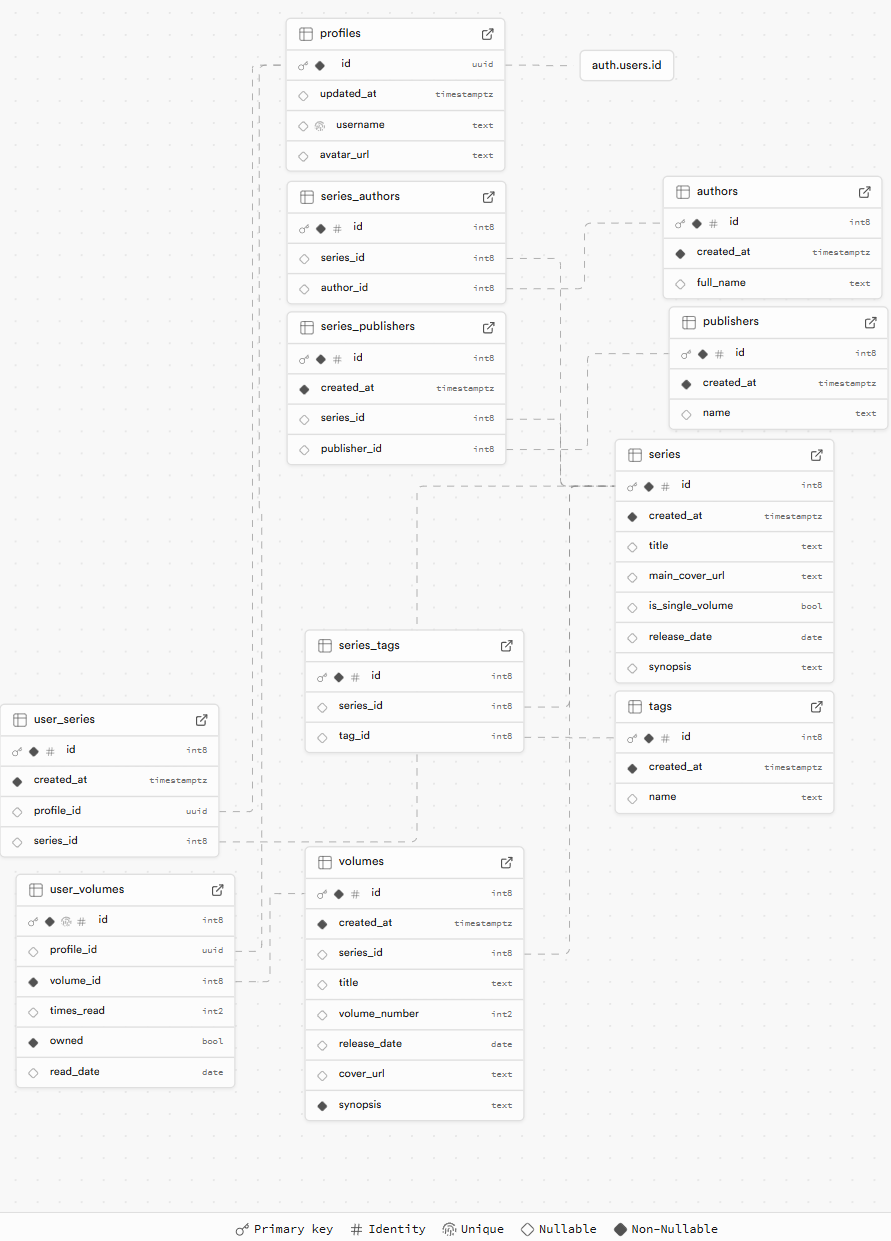
\includegraphics[width=1\textwidth]{figures/schemat1.png}
	\caption{Schemat bazy danych}
\label{Fig:schemat}
\end{figure}

\clearpage

\subsubsection{Normalizacja}

Normalizacja bazy danych to proces organizowania danych w taki sposób, aby zminimalizować redundancję i zapewnić 
integralność danych. Celem jest poprawienie struktury bazy w sposób, który ułatwia jej zarządzanie i utrzymanie, 
eliminując potencjalne problemy związane z nieefektywnym przechowywaniem informacji.

\begin{enumerate}[label=\alph*), leftmargin=1.25cm]
	\item pierwsza postać normalna (1NF) na podstawie kodu z listingu \ref{publicSeries}
	\begin{lstlisting}[language=SQL,caption=kod tworzenia tabeli series, label={publicSeries}]
		CREATE TABLE public.series (
			id bigint GENERATED BY DEFAULT AS IDENTITY NOT NULL,
			title text NULL,
			...
			CONSTRAINT Series_pkey PRIMARY KEY (id)
		  );
		\end{lstlisting}
		Tabela series spełnia pierwszą postać normalną, ponieważ kolumny takie jak title zawierają atomowe 
		wartości, a klucz główny (id) zapewnia unikalność każdego rekordu,

	\item druga postać normalna (2NF) na podstawie kodu z listingu \ref{publicVolumes}
	\begin{lstlisting}[language=SQL,caption=kod tworzenia tabeli volumes, label={publicVolumes}]
		CREATE TABLE public.volumes (
			id bigint GENERATED BY DEFAULT AS IDENTITY NOT NULL,
			series_id bigint NULL,
			title text NULL,
			...
			CONSTRAINT volumes_pkey PRIMARY KEY (id),
			CONSTRAINT volumes_series_id_fkey FOREIGN KEY (series_id) REFERENCES series(id)
	 	 );
		\end{lstlisting}
		Tabela volumes spełnia drugą postać normalną, ponieważ jest w pierwszej postaci normalnej oraz 
		wszystkie kolumny, które nie są częścią klucza głównego, są w pełni zależne od klucza głównego (id). 
		Kolumna series\_id jest kluczem obcym, a kolumny jak title zależą od id, co eliminuje zależności 
		częściowe,
	
	\item trzecia postać normalna (3NF) na podstawie kodu z listingu \ref{publicUserSeries}
	\begin{lstlisting}[language=SQL,caption=kod tworzenia tabeli user\_series, label={publicUserSeries}]
		CREATE TABLE public.user_series (
			id bigint GENERATED BY DEFAULT AS IDENTITY NOT NULL,
			profile_id uuid NULL,
			series_id bigint NULL,
			...
			CONSTRAINT user_series_pkey PRIMARY KEY (id),
			CONSTRAINT user_series_profile_id_fkey FOREIGN KEY (profile_id) REFERENCES profiles(id),
			CONSTRAINT user_series_series_id_fkey FOREIGN KEY (series_id) REFERENCES series(id)
	  );
		\end{lstlisting}
		Tabela user\_series spełnia trzecią postać normalną, ponieważ jest w drugiej postaci normalnej, a 
		dodatkowo nie występują zależności przejściowe. Kolumny, które nie są częścią klucza głównego, zależą 
		tylko od klucza głównego (id), a nie od innych kolumn, co zapewnia brak zbędnych zależności między danymi.
		Tabela ta spełnia również BCNF, ponieważ każda kolumna w niej zależy bezpośrednio od głównego identyfikatora 
		(id),
	
	\item czwarta postać normalna (4NF) na podstawie kodu z listingu \ref{publicSeriesAuthors}
	\begin{lstlisting}[language=SQL,caption=kod tworzenia tabeli series\_authors, label={publicSeriesAuthors}]
		CREATE TABLE public.series_authors (
		id bigint GENERATED BY DEFAULT AS IDENTITY NOT NULL,
		series_id bigint NULL,
		author_id bigint NULL,
		CONSTRAINT series_author_pkey PRIMARY KEY (id),
		CONSTRAINT series_author_author_id_fkey FOREIGN KEY (author_id) REFERENCES authors(id) ON UPDATE CASCADE ON DELETE CASCADE,
		CONSTRAINT series_author_series_id_fkey FOREIGN KEY (series_id) REFERENCES series(id) ON UPDATE CASCADE ON DELETE CASCADE
	);
	\end{lstlisting}
	Tabela series\_authors spełnia czwartą postać normalną, ponieważ nie zawiera zależności wielowartościowych. Relacja 
	między series\_id a author\_id jest wyrażona w sposób atomowy, gdzie każda kombinacja serii i autora jest 
	reprezentowana przez pojedynczy wiersz. Tabela nie wprowadza redundancji związanej z wieloma wartościami 
	przypisanymi do jednej kolumny
\end{enumerate}


\subsection{Funkcje bazy danych}

Funkcje bazy danych stanowią ważny element w zarządzaniu danymi, umożliwiając efektywne wykonywanie różnych operacji 
w obrębie samej bazy danych. Funkcje PostgreSQL pozwalają na grupowanie złożonych zapytań, usprawnienie przetwarzania 
danych oraz zwiększenie wydajności operacji. Dzięki funkcjom bazy danych możliwe jest wykonywanie operacji 
specyficznych dla aplikacji bezpośrednio na poziomie bazy danych, co pozwala na zmniejszenie obciążenia aplikacji i 
serwera.

Kod przykładowej funkcji bazy danych znajduje się w listingu \ref{sqlFunction}

	\begin{lstlisting}[language=SQL,caption=kod funkcji get\_volume\_by\_id, label={sqlFunction}]
		CREATE OR REPLACE FUNCTION public.get_volume_by_id(p_volume_id bigint)
		RETURNS TABLE(id bigint, title text, cover_url text, volume_number smallint, user_volume_id bigint, release_date timestamp with time zone, times_read smallint, owned boolean, synopsis text, read_date timestamp with time zone)
		LANGUAGE plpgsql
	   AS $function$
	   BEGIN
		   RETURN QUERY
		   SELECT 
			   v.id,
			   v.title,
			   v.cover_url,
			   v.volume_number,
			   uv.id AS user_volume_id,
			   v.release_date,
			   COALESCE(uv.times_read, 0) AS times_read,
			   COALESCE(uv.owned, false) AS owned,
			   v.synopsis,
			   uv.read_date
		   FROM 
			   volumes v
		   LEFT JOIN 
			   user_volumes uv ON v.id = uv.volume_id
		   WHERE 
			   v.id = p_volume_id;
	   END;
	   $function$;
	\end{lstlisting}

funkcja ta pozwala na podstawie identyfikatora pobrać z bazy danych informacje o wybranym tomie książki (volume), z bazy
danych. Funkcja zwraca wynik w postaci teabeli zawierającej dane o tomie oraz dodatkowe informacje związane z użytkownikiem
jeżeli są dostępne, takie jak pobrane z tabeli user\_volumes, times\_read informujące o tym ile razy użytkownik przeczytał
dany tom. Może wystąpić sytuacja, w której pobierany tom nie ma odpowiadającego rekordu w tabeli user\_volumes, ponieważ 
użytkownik nie oznaczył go jako przeczytanego ani posiadanego. W takim przypadku dane użytkownika zostaną uzupełnione 
domyślnymi wartościami, takimi jak 0 dla liczby przeczytań czy false dla statusu posiadania, co jest zrealizowane z 
wykorzystaniem funkcji COALESCE, której użycie można zaobserować w liniach 14 i 15.

\clearpage

\section{Architektura i struktura aplikacji}

Architektura aplikacji została oparta na wzorcu MVVM, co pozwala na efektywne zarządzanie stanem i separację 
logiki biznesowej od interfejsu użytkownika. Właściwa organizacja plików w projekcie jest kluczowa dla 
utrzymania porządku i skalowalności aplikacji, umożliwiając łatwe zarządzanie komponentami i ich zależnościami. 

\subsection{Struktura projektu}

Aplikacja została wykonana z wykorzystaniem narzędzia Android Studio, a struktura projektu została zaprojektowana 
zgodnie z rekomendowanymi zasadami architektury MVVM (Model-View-ViewModel), co zapewnia czytelność, modułowość
oraz łatwość w utrzymaniu i rozwoju kodu. Struktura plików projektu przedstawiona jest na rysunku \ref{Fig:struktura}

\begin{figure}[ht]
	\centering
	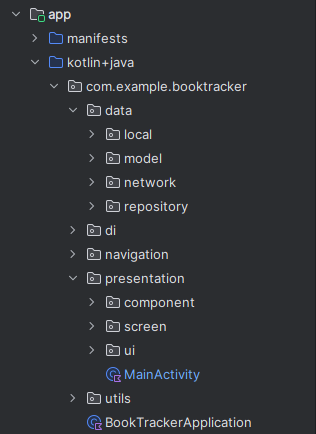
\includegraphics{figures/struktura.png}
	\caption{Struktura plików aplikacji}
\label{Fig:struktura}
\end{figure}

\subsubsection{Folder data}

Folder data pełni rolę zbiorczą dla klas i funkcji odpowiedzialnych za zarządzanie danymi, w tym ich przechowywanie 
oraz pobieranie z bazy danych.

\begin{enumerate}[label=\alph*), leftmargin=1.25cm]
	\item Folder local jest przeznaczony do przechowywania danych lokalnych, takich jak tokeny autoryzacyjne, 
	ustawienia aplikacji czy inne informacje, które nie wymagają zdalnej synchronizacji, z wykorzystaniem biblioteki 
	DataStore, która zapewnia bezpieczne i efektywne przechowywanie danych w formie klucz-wartość lub preferencji,
	\item Folder model służy do przechowywania klas DTO (Data Transfer Object), które są serializowanymi obiektami 
	wykorzystywanymi do przechowywania danych pobranych z bazy danych. Klasom tym przypisuje się odpowiednie 
	struktury, które umożliwiają prawidłowe reprezentowanie i manipulowanie danymi w aplikacji,
	\item w folderze network przechowywane są klasy DAO (Data Access Object), które odpowiadają za komunikację z 
	bazą danych Supabase. Klasy te pełnią rolę abstrakcji, umożliwiając wykonywanie operacji na danych, takich jak 
	pobieranie, zapisywanie czy aktualizowanie rekordów, bezpośrednio w bazie. Dzięki zastosowaniu wzorca DAO, 
	operacje te są oddzielone od logiki aplikacji, co zapewnia lepszą modularność, łatwiejsze zarządzanie dostępem do 
	danych oraz umożliwia łatwiejszą wymianę technologii dostępu do danych w przyszłości,
	\item Folder repository jest odpowiedzialny za przechowywanie klas repozytoriów, które pełnią rolę pośredników 
	pomiędzy warstwą danych a resztą aplikacji. Repozytoria w tym folderze odpowiadają za realizację operacji dostępu 
	do różnych źródeł danych. Oddzielają one logikę biznesową aplikacji od szczegółów technicznych, zapewniając 
	łatwiejsze zarządzanie danymi oraz umożliwiając przyszłe zmiany w źródłach danych bez wpływu na resztę aplikacji. 
	Repozytoria ułatwiają testowanie, zapewniają modularność aplikacji i poprawiają jej elastyczność, umożliwiając 
	łatwą wymianę technologii dostępu do danych.
\end{enumerate}

\subsubsection{Folder di (Dependency Injection)}

Folder di służy do przechowywania modułów odpowiedzialnych za konfigurację zależności aplikacji. Wykorzystuje 
bibliotekę Hilt, która umożliwia definiowanie sposobu tworzenia i dostarczania wymaganych obiektów, takich jak 
klienty API, repozytoria czy inne kluczowe komponenty. Moduły w tym folderze zapewniają centralne miejsce do 
zarządzania zależnościami, co ułatwia organizację projektu i poprawia czytelność kodu.

\subsubsection{Folder navigation}

Folder navigation zarządza całą logiką nawigacji w aplikacji, co umożliwia łatwe i efektywne przejścia pomiędzy 
ekranami. Zawiera definicję ekranów jako obiektów typu sealed class, co pozwala na centralne zarządzanie wszystkimi 
dostępnymi widokami w aplikacji. W tym folderze określane są także zasady dotyczące tego, kiedy i jak ekran powinien 
wyświetlać dodatkowe komponenty, takie jak dolne menu nawigacyjne.

Dzięki wykorzystaniu biblioteki navigation-compose, folder navigation umożliwia łatwą konfigurację tras i przejść, 
eliminując konieczność ręcznego zarządzania stanem nawigacji. Obsługuje różne scenariusze, takie jak logowanie, 
rejestracja, przeglądanie biblioteki czy edycja profilu użytkownika, zapewniając płynność i spójność w nawigacji. 
W połączeniu z komponentem NavHost, aplikacja może efektywnie zarządzać stanem nawigacyjnym, przechodzić między 
ekranami i dostosowywać animacje przejść. Dzięki tej strukturze, aplikacja jest bardziej modularna, a logika 
nawigacyjna pozostaje łatwa do utrzymania i rozbudowy.

\subsubsection{Folder presentation}



\subsubsection{Folder utils}

Folder utils zawiera funkcje pomocnicze, które wspierają różne operacje w aplikacji, takie jak walidacja danych 
wejściowych. Funkcje te są uniwersalne i mogą być wykorzystywane w różnych częściach projektu, co pozwala na unikanie 
powielania kodu. Dzięki temu zapewniają one centralizację logiki, co ułatwia utrzymanie aplikacji, poprawia jej 
czytelność oraz umożliwia łatwiejsze testowanie. Przykłady funkcji w tym folderze to metody sprawdzające poprawność 
adresu e-mail, hasła czy nazwy użytkownika. Wszystkie funkcje w utils są zaprojektowane w sposób modularny, co 
pozwala na ich elastyczne zastosowanie w całym projekcie. Przykładowa funkcja znajduje się listingu \ref{validateEmail}

\begin{lstlisting}[language=Kotlin,caption=kod funkcji validateEmail, label={validateEmail}]
	fun validateEmail(email: String, context: Context): String? {
    	val emailRegex = "^[A-Za-z0-9+_.-]+@[A-Za-z0-9.-]+\$".toRegex()
    		return if (email.isEmpty()) {
        		context.getString(R.string.email_empty)
    		} else if (!email.matches(emailRegex)) {
        		context.getString(R.string.invalid_email)
    		} else null
		}
\end{lstlisting}

\subsection{MVVM (Model-View-ViewModel)}

Model-View-ViewModel to popularny wzorzec architektoniczny stosowany w tworzeniu aplikacji, który pomaga w 
organizacji kodu i rozdzieleniu odpowiedzialności pomiędzy różne warstwy aplikacji. Jego głównym celem
jest zwiększenie modularności, łatwości testowania oraz oddzielenie logiki biznesowej od interfejsu użytkownika.

\begin{enumerate}[label=\alph*), leftmargin=1.25cm]
	\item Model reprezentuje warstwę danych i logiki biznesowej. Jest odpowiedzialny za zarządzanie danymi,
	które mogą pochodzić z różnych źródeł, takich jak bazy danych, API czy pliki lokalne. Model nie zawiera
	żadnej logiki związanej z interfejsem użytkownika ani sposobem prezentacji danych,
	\item View (Widok) odpoawiada za warstwę prezentacji. Widok to interfejs użytkownika (UI), który jest
	odpowiedzialny za wyświetlenie danych i odbieranie interakcji od użytkownika. Widok powinien jedynie
	reagować na dane dostarczane przez ViewModel. W android widokiem są komponenty Jetpack Compose,
	\item ViewModel to warstwa pomiędzy modelem a widokiem. pobiera dane z modelu i przekształca je
	w taki sposób, aby były gotowe do wyświetlenia w widoku. Ponadto zarządza stanem widoku (np. przechowywaniem
	stanu aplikacji w przypadku zmiany orientacji ekranu).
\end{enumerate}

\subsubsection{Model}

W poniższym listingu 

\clearpage

\addcontentsline{toc}{section}{Literatura}

\begin{thebibliography}{4}
\end{thebibliography}

\clearpage

\makesummary

\end{document} 
